%%%%%%%%%%%%%%%%%%%%%%%%%%%%%%%%%%%%%%%%%%%%%%%%%%%%%%%%%%%%%%%%%%%%
%% I, the copyright holder of this work, release this work into the
%% public domain. This applies worldwide. In some countries this may
%% not be legally possible; if so: I grant anyone the right to use
%% this work for any purpose, without any conditions, unless such
%% conditions are required by law.
%%%%%%%%%%%%%%%%%%%%%%%%%%%%%%%%%%%%%%%%%%%%%%%%%%%%%%%%%%%%%%%%%%%%

% This theme was based on fibeamer theme 
% If you found any bugs please contact @karlosos
% This repository is hosted on github https://github.com/karlosos/zut-fibeamer/

\documentclass{beamer}
\usetheme[faculty=wi]{fibeamer}
\usepackage[utf8]{inputenc}
\usepackage[
  main=english,
  english
]{babel}


\includegraphics[width=0.5\textwidth]{fibeamer/logo/zut/logo.png}
\title{Graph Convolutional Networks for Text Classification}
\subtitle{A paper by L. Yao, C. Mao, and Y. Lua, 2019}
% \author{Author's Name}

\usepackage{ragged2e}  % `\justifying` text
\usepackage{booktabs}  % Tables
\usepackage{tabularx}
\usepackage{tikz}      % Diagrams
\usetikzlibrary{calc, shapes, backgrounds}
\usepackage{amsmath, amssymb}
\usepackage{url}       % `\url`s
\usepackage{listings}  % Code listings
\usepackage{graphicx}

\frenchspacing
\begin{document}
  \frame[c]{\maketitle}
  \AtBeginSection[]{% Print an outline at the beginning of sections
    \begin{frame}<beamer>
      \frametitle{Outline for Section \thesection}
    %   \tableofcontents[currentsection]
    \end{frame}}

  \begin{darkframes}

    \begin{frame}[label=lists]{Text classification}
        \framesubtitle{Why?}
        \textit{News filtering},\clearpage
        \textit{Spam detection},\clearpage
        \textit{Opinion mining},\clearpage
        \textit{and much more...}\clearpage
        But!\clearpage
        Before training a model on textual data, one must first pre-process it.
    \end{frame}

    \begin{frame}[label=lists]{Text representation}
        \framesubtitle{Text can be processed into array representations: Embeddings}
        \centering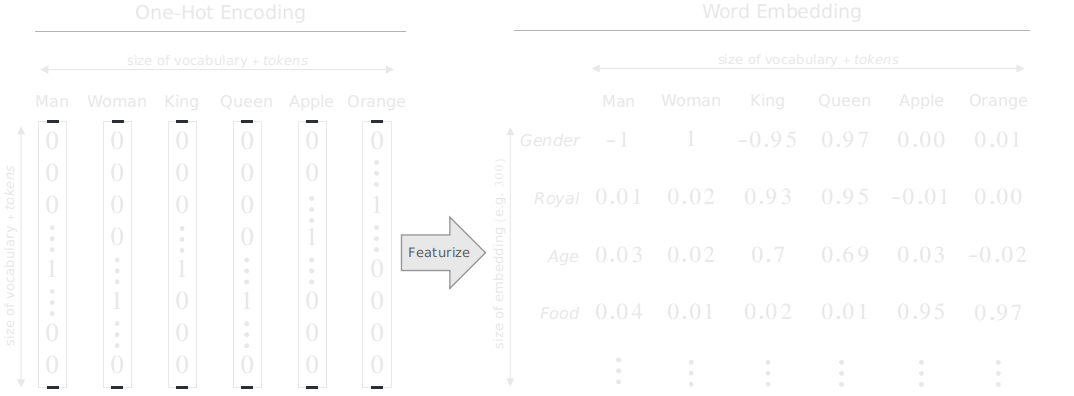
\includegraphics[width=\textwidth]{fibeamer/logo/zut/embeds.png}
        \clearpage
        \raggedright\textit{It is the main method used today: to embed text features in an array (e.g. via a pre-trained model like GloVe)}.
        \clearpage
        \raggedright\tiny{Ng, Andrew. \emph{NLP and Word Embeddings, deeplearning.ai, 2021}}
    \end{frame}

    \begin{frame}[label=lists]{}
        \large{So... convolution? How?}
    \end{frame}
    
    \begin{frame}[label=lists]{Convolution}
        \framesubtitle{An image is an array}
        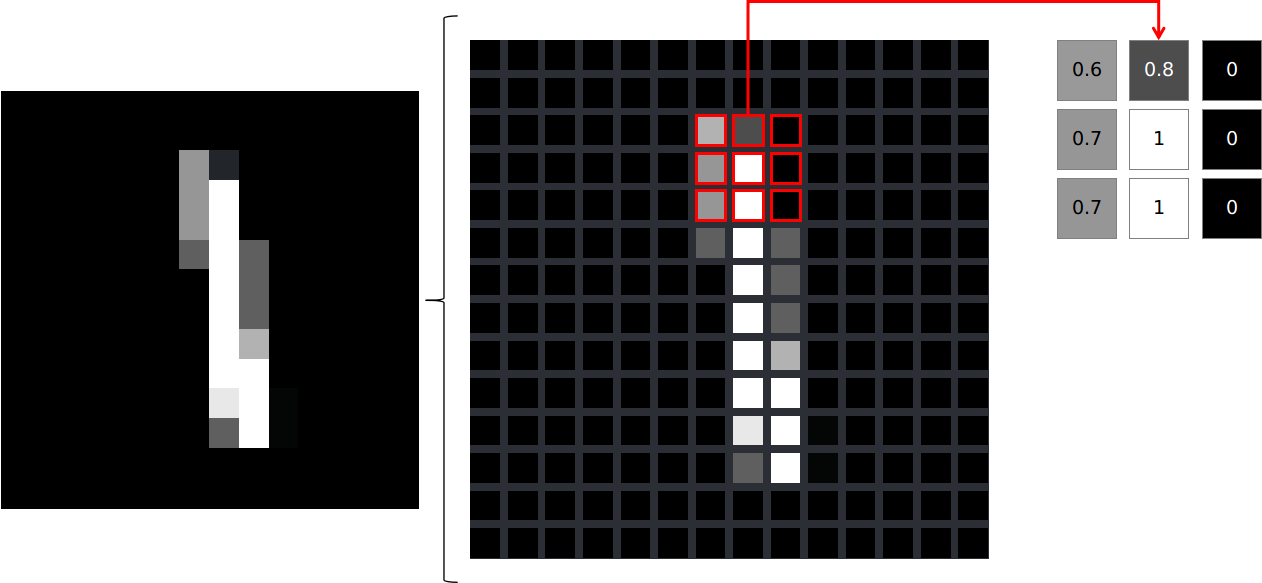
\includegraphics[width=\textwidth]{fibeamer/logo/zut/convolution.png}
        Using an example from MNIST.
        \clearpage
        \raggedright\tiny{Le Cun, Yann. The MNIST database of handwritten digits, 1998}
    \end{frame}

    \begin{frame}[label=lists]{Convolution}
        \framesubtitle{We can perform computation on window-snippets of the array}
        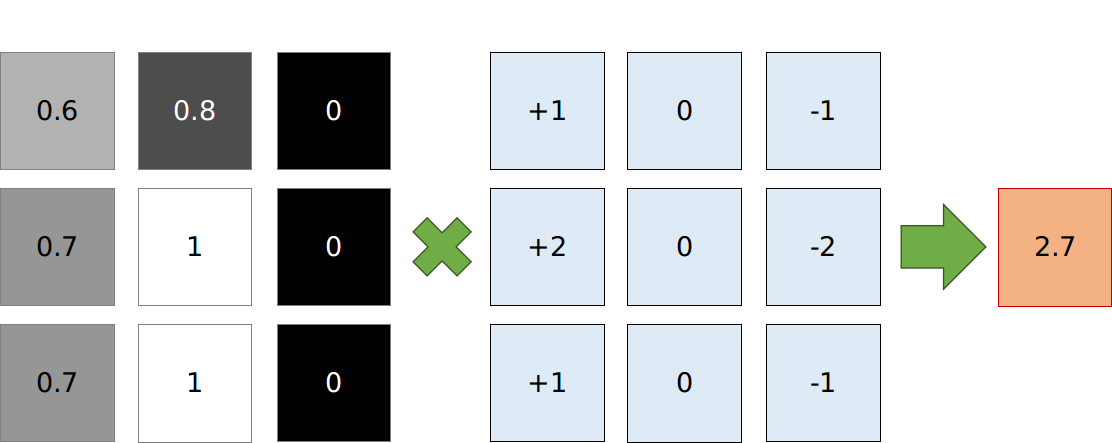
\includegraphics[width=\textwidth]{fibeamer/logo/zut/sobel.png}
    \end{frame}
    
    \begin{frame}[label=lists]{Convolution}
        \framesubtitle{Pictures can be represented as something else: Graphs...}
        \centering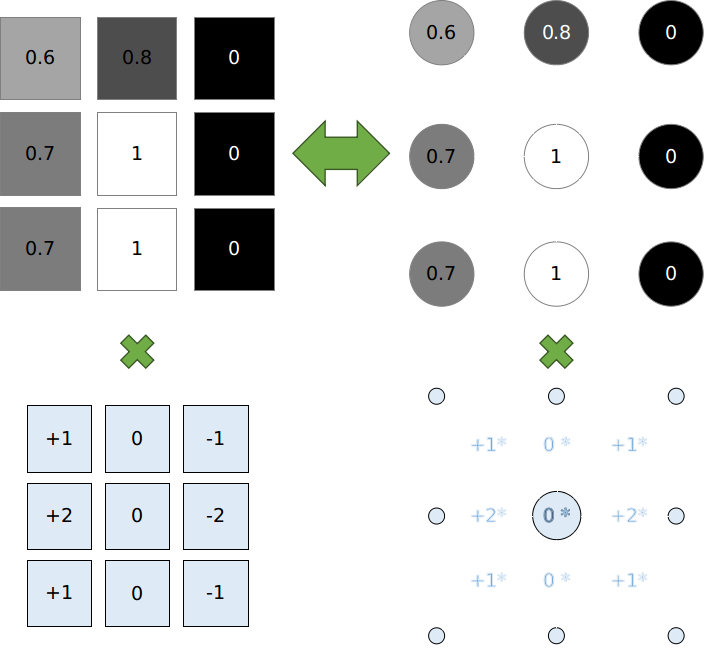
\includegraphics[width=0.56\textwidth]{fibeamer/logo/zut/correspondance.png}\\
        It means convolution does not only apply to pictures and signals.
    \end{frame}
    
    \begin{frame}[label=lists]{Convolution}
        \framesubtitle{... and graphs can be used as inputs to neural networks}
        \centering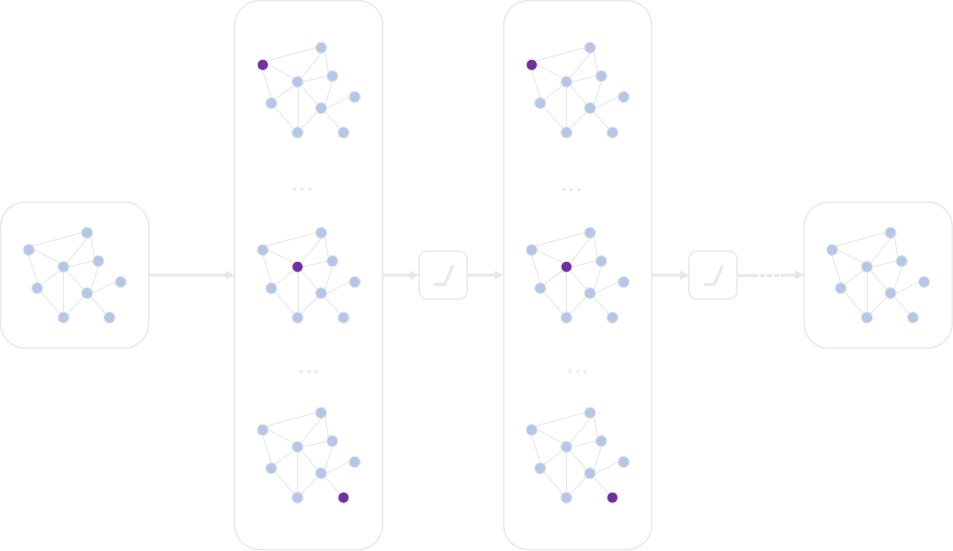
\includegraphics[width=0.9\textwidth]{fibeamer/logo/zut/graph.png}
        \clearpage
        \raggedright\tiny{Kipf, Thomas N. and Welling, Max. \emph{Semi-Supervised Classification with Graph Convolutional Networks, ICLR, 2017}}
    \end{frame}

    \begin{frame}[label=lists]{\large{Graph Convolutional Networks for Text Classification}}
        % \framesubtitle{}
        Graph neural networks, and graph embeddings are recent.
        \clearpage
        They offer a richer relational representation than CNN and RNN, giving less priority to locality and sequentiality.\clearpage
        They capture a \underline{higher order neighborhood information}.
        \clearpage
        \clearpage
        $\Rightarrow$ The paper at hand proposes a new graph neural network method for text classification.
        \clearpage
        \clearpage
        \raggedright\tiny{Battablia et al. \emph{Relational inductive biases, deep learning, and graph networks, 2018}}\\
        \raggedright\tiny{Yao, L., Mao, C., Luo, Y. \emph{Graph Convolutional Networks for Text Classification, 2019}}
    \end{frame}
    
    \begin{frame}[label=lists]{\large{Graph Convolutional Networks for Text Classification}}
        \framesubtitle{How to construct a graph}
        \underline{Usual ML solution:} builds a word or document embedding.\\
        \underline{Graph neural network solution:} learns both at once.
        \clearpage
        \clearpage
        It relies on a \textbf{non-grid} or \textbf{arbitrarily structured graph}:\\
        \quad - Nodes represents words \underline{or} document types\\
        \quad - Edges represent co-occurrences
        \clearpage
        \clearpage
        $\Rightarrow$ Text \underline{and} document classification is a node classification problem
        \clearpage
        \clearpage
        \raggedright\tiny{Bruna, J. et al. \emph{Spectral Networks and Locally Connected Networks on Graphs, 2014}}
    \end{frame}
    
    \begin{frame}[label=lists]{\large{Graph Convolutional Networks for Text Classification}}
        \framesubtitle{A 2-Layer Graph Convolutional Network}
        \begin{figure}[h!]
          \centering
          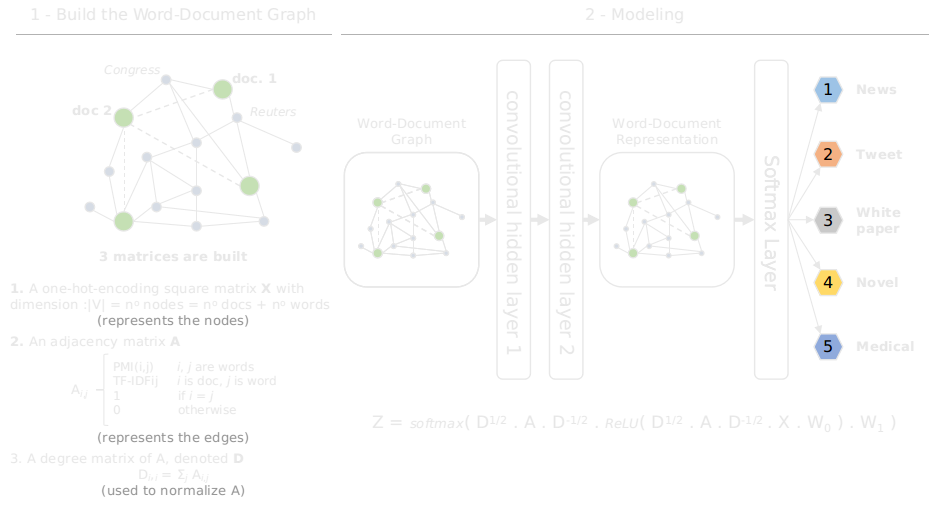
\includegraphics[width=\textwidth]{fibeamer/logo/zut/model.png}
        \end{figure}
        \raggedright\tiny{\textbf{Note}: A fixed size sliding window on all documents in the corpus is used to gather co-occurrence statistics.\\
        \textbf{TF-IDF}: term frequency-inverse document frequency; \textbf{PMI}: point-wise mutual information}
    \end{frame}
    
    \begin{frame}[label=lists]{\large{Graph Convolutional Networks for Text Classification}}
        \framesubtitle{Datasets}
        \footnotesize{\begin{center}
        \begin{tabular}{ c c c c c c c }
         Name & Content & \# Docs & Split & \# Words & \# Nodes & \# Classes  \\ 
         \hline
         20NG & News slips & 18,846 & 60-40 & 42,757 & 61,603 & 20 \\  
         R8 & Reuters cables & 7,674 & 70-30 & 7,688 & 15,362 & 8 \\ 
         R52 & Reuters cables & 9,100 & 71-29 & 8,892 & 17992 & 52 \\ 
         Ohsumed & Medical lit. & 7,400 & 45-55 & 14,157 & 21,557 & 23 \\ 
         MR & Movie reviews & 10,662 & 67-33 & 18,764 & 29,426 & 2
        \end{tabular}
        \end{center}}
        \clearpage
        \underline{Embedding size of the first convolutional layer:} 200
        \\\underline{Window size:} 20
        \clearpage
        \underline{The paper's main question:} 
        \clearpage
        \centering Can the model achieve satisfactory results in text classification, even with limited labeled data?
        \clearpage
    \end{frame}
    
    \begin{frame}[label=lists]{\large{Graph Convolutional Networks for Text Classification}}
        \framesubtitle{Results}
        \footnotesize{
        \centering\caption{\textit{Mean test accuracy - Models were run 10 times}}
        \begin{center}
        \begin{tabular}{ c c c c c c c }
         Models & 20NG & R8 & R52 & Ohsumed & MR \\
         \hline
         Text GCN & \textcolor{green}{$0.86$} & \textcolor{green}{$0.97$} & \textcolor{green}{$0.94$} & \textcolor{green}{$0.68$} & $0.77$ \\
         SWEM & $0.85$ & $0.95$ & $0.93$ & $0.63$ & $0.77$ \\
         TF-IDF + LogReg & $0.83$ & $0.94$ & $0.87$ & $0.55$ & $0.75$ \\
         CNN & $0.82$ & $0.96$ & $0.88$ & $0.58$ & \textcolor{green}{$0.78$} \\
         LEAM & $0.82$ & $0.93$ & $0.92$ & $0.59$ & $0.77$ 
        \end{tabular}
        \end{center}}
        \centering"\textbf{Text GCN performs the best and significantly outperforms all baseline models}."\\
        
        \clearpage
        \raggedright\tiny{\textbf{Note}: 12 models were omitted from this table. \\\textbf{SWEAM}: Simple Word Embedding Model. \textbf{LEAM}: Label-Embedding Attentive Model.}
    \end{frame}
    
    \begin{frame}[label=lists]{\large{Graph Convolutional Networks for Text Classification}}
        \framesubtitle{Further results}
        \centering Text GCN can capture both document-to-word and global word-to-word relations.
        \clearpage
        \centering Word nodes capture document label information and act as bridges: label information propagates across the graph.
        \clearpage
        \centering Text GCN does not outperform CNN and LSTM on the MR dataset: Text GCN \textit{ignores word order}, a key feature in sentiment analysis.
        \clearpage
    \end{frame}

    \begin{frame}[label=lists]{\large{Formulas}}
        TF-IDF:
        $$\frac{{\# word\,occurrences\,in\,the\,document}}{log({\#\,of\,documents\,that\,contain\,the\,word})}$$
        PMI:
        \footnotesize{$${PMI}(i, j) = {log}\frac{p(i, j)}{p(i)p(j)}$$
        $$p(i, j) = \frac{\#W(i, j)}{\#W}$$
        $$p(i) = \frac{\#W(i)}{\#W}$$
        with $\#W(i)$, the number of sliding windows in a corpus that contains word i, $\#W(i, j)$, the number of sliding windows that contain both words i and j, and $\#W$ the total number of sliding windows.}
    \end{frame}

    \subsection{Citations and Bibliography}
    
    \begin{frame}[label=bibliography]{Bibliography}
      \begin{thebibliography}{9}
        \scriptsize{
        \bibitem{ng}
            Ng, Andrew.
            \emph{NLP and Word Embeddings - CS230 Deep Learning, Stanford University}.
            deeplearning.ai, 2021.
        \bibitem{lecun}
            Le Cun, Yann.
            \emph{The MNIST database of handwritten digits}.
            1998.
        \bibitem{kipf2017semi}
            Kipf, Thomas N. and Welling, Max.
            \emph{Semi-Supervised Classification with Graph Convolutional Networks}.
            International Conference on Learning Representations (ICLR), 2017.
        \bibitem{battaglia2018relational}
            Battaglia, P. et al.
            \emph{Relational inductive biases, deep learning, and graph networks}. 2018.
        \bibitem{bruna2014spectral}
            Bruna, J. et al.
            \emph{Spectral Networks and Locally Connected Networks on Graphs}. 2014.
        }
        
        
      \end{thebibliography}
    \end{frame}
\end{darkframes}

\end{document}